\documentclass[a4paper,12pt]{report}

% Pacotes necessários
\usepackage[utf8]{inputenc}      % Suporte para caracteres UTF-8
\usepackage[T1]{fontenc}         % Codificação de fonte
\usepackage[portuguese]{babel}   % Suporte ao português
\usepackage{graphicx}            % Inclusão de imagens
\usepackage{float}               % Controle de posicionamento de figuras
\usepackage{amsmath}             % Matemática avançada
\usepackage{listings}            % Para incluir códigos-fonte
\usepackage{hyperref}            % Links no PDF
\usepackage{geometry}            % Configuração da página
\usepackage{booktabs}            % Tabelas mais elegantes
\usepackage[pdf]{graphviz}
\usepackage{subfigure}
\usepackage{setspace}
\geometry{a4paper, margin=2.5cm}

% Configuração para código-fonte
\lstset{
  language=C,
  basicstyle=\small,
  captionpos=b,
  float=tp,
  xleftmargin=1.5em,
  xrightmargin=1.5em,
  frameround=ttff,
  frame=single,
  floatplacement=tbp
}

% Informações de título
\title{%
  \textbf{Relatório do Trabalho Prático}\\[4em]
  \large Laboratórios de Informática \\[4em]
  Licenciatura em Engenharia de Sistemas Informáticos -- 2024/25
}
\author{Grupo G06}
\date{\today}

\begin{document}

% Capa
\maketitle

\tableofcontents
\listoffigures
\listoftables

\chapter{Introdução}
Este relatório descreve o desenvolvimento do trabalho prático para a unidade curricular Laboratórios de Informática. O objetivo é implementar uma aplicação em C para a gestão de um espaço social, aplicando boas práticas de programação, modularização e automação. Este relatório segue a estrutura recomendada no enunciado.

\chapter{Objetivos}
O principal objetivo é a prática de desenvolvimento em grupo de um sistema usando C e ferramentas associadas. Os sub-objetivos incluem:
\begin{itemize}
    \item Modularização do código em arquivos separados.
    \item Automação do processo de compilação com \texttt{Makefile}.
    \item Controlo de versão utilizando o GitHub.
    \item Criação de relatórios estruturados em LaTeX.
\end{itemize}

\chapter{Desenvolvimento}

\section{Descrição do Problema}
A aplicação tem como objetivo a gestão de um espaço social, com funcionalidades como:
\begin{itemize}
    \item Registar e gerir informações de funcionários.
    \item Registar e exibir ementas semanais.
    \item Registar as escolhas alimentares dos funcionários.
    \item Fornecer análises.
    \item Manter tabelas organizadas e atualizadas.
\end{itemize}

\section{Estrutura do Código}
O projeto foi estruturado em pastas e arquivos para modularização:

\begin{itemize}
    \item \textbf{src/}: Código-fonte.
    \item \textbf{doxdoc/}: Documentação do Doxyfile.
    \item \textbf{doc/}: Documentação e relatórios.
\end{itemize}

\break

\section{Makefile}
Este é um ficheiro \texttt{Makefile}, escrito para que o processo de compilação de um documento LaTeX seja automático. 

\begin{figure}[H]
    \centering
    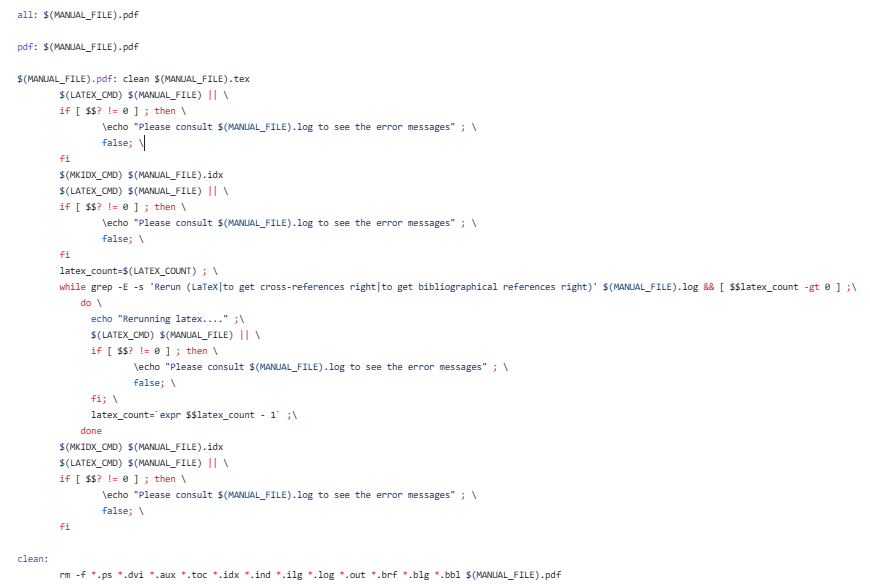
\includegraphics[width=\linewidth]{image.png}
    \caption{Exemplo do ficheiro Makefile}
    \label{fig:makefile}
\end{figure}

\section{Documentação com Doxygen}
O Doxygen foi utilizado para gerar documentação do código, com suporte a HTML e PDF.
Estes foram os comandos utilizados para fazer a documentação doxygen:
\begin{itemize}
    \item doxygen -g Doxyfile 
    \item doxygen Doxyfile
\end{itemize}

\begin{figure}[H]
    \centering
    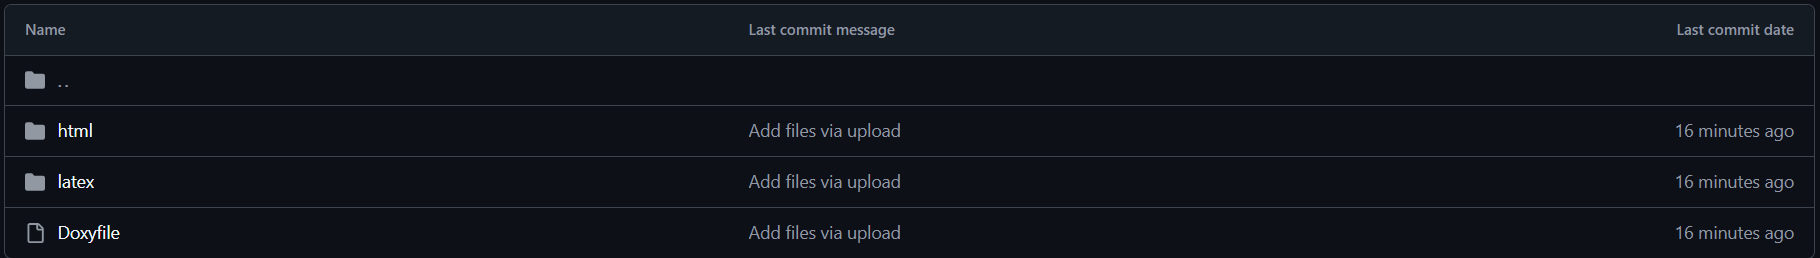
\includegraphics[width=\linewidth]{doxygen.png}
    \caption{Exemplo da documentação com Doxygen}
    \label{fig:doxygen}
\end{figure}

\break

\section{Controlo de Versão}
O repositório foi criado no GitHub, com as pastas organizadas para cada funcionalidade. O fluxo de trabalho seguiu a prática de pull requests.

\begin{figure}[H]
    \centering
    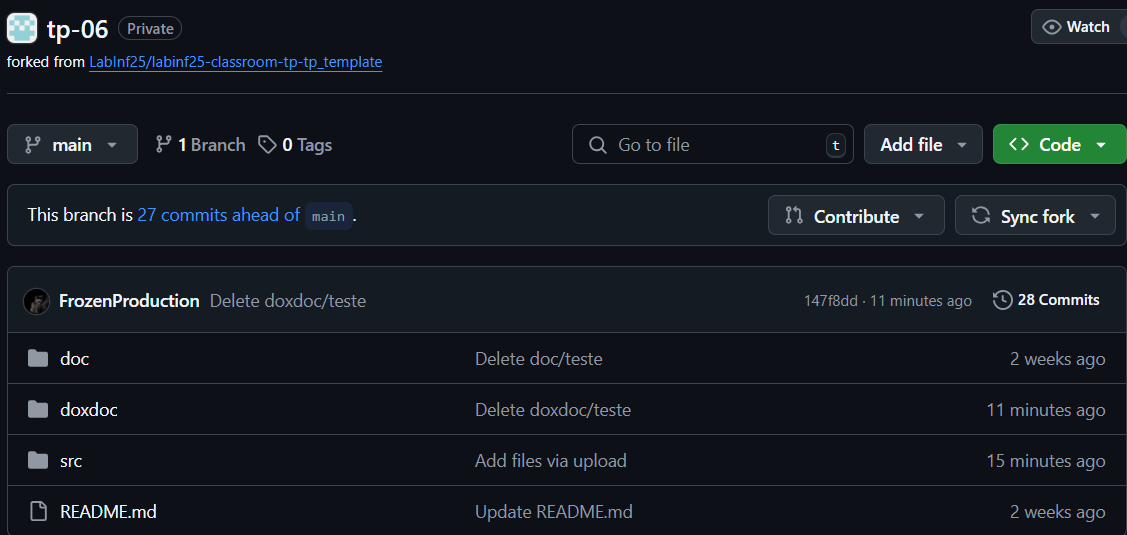
\includegraphics[width=\linewidth]{controlo_de_versao.png}
    \caption{Exemplo do Repositório no GitHub}
    \label{fig:github}
\end{figure}

\chapter{Resultados}

\section{Funcionamento}
Os principais módulos desenvolvidos incluem:
\begin{itemize}
    \item \textbf{Consulta e Exibição de Dados}: Listagem dos funcionários e visualização das ementas.
    \item \textbf{Ordenação e Atualização}: Ordenação dos funcionários por ordem decrescente e atualização dos funcionários e das suas ementas.
    \item \textbf{Relatórios e Estatísticas}: Relatórios de consumo e cálculo da média de calorias consumidas por dia.
    \item \textbf{Filtros e Pesquisas}: Pesquisa das refeições de um funcionário.
\end{itemize}

\section{Tabelas}
A tabela abaixo resume as refeições de um dia da semana:
\begin{table}[H]
    \centering
    \begin{tabular}{lccc}
    \toprule
    \textbf{Nº Func.} & \textbf{Nome} & \textbf{Tipo de Prato} \\
    \midrule
    1 & Paulo Silva & D \\
    3 & Maria João Pires & C \\
    4 & Ana Carvalho & V \\
    \bottomrule
    \end{tabular}
    \caption{Exemplo das refeições para um dia da semana.}
    \label{tab:refeicoes_dia}
\end{table}

Esta tabela representa a lista de funcionários:
\begin{table}[H]
    \centering
    \begin{tabular}{lccc}
    \toprule
    \textbf{Nº Func.} & \textbf{Nome} & \textbf{NIF} & \textbf{Telefone} \\
    \midrule
    1 & Paulo Silva & 179204181123456789 & 123456789 \\
    2 & João Cunha & 178781342987654321 & 987654321 \\
    3 & Maria João Pires & 173456789912345678 & 912345678 \\
    4 & Ana Carvalho & 204168169965432101 & 965432101 \\
    \bottomrule
    \end{tabular}
    \caption{Exemplo da lista de funcionários.}
    \label{tab:lista_funcionarios}
\end{table}

Esta tabela contém as informações sobre os pratos disponíveis:
\begin{figure}[H]
    \centering
    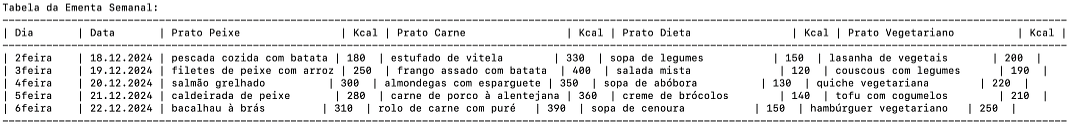
\includegraphics[width=\linewidth]{imagem_tabela.png}
    \caption{Exemplo das refeições semanais.}
    \label{fig:refeicoes_semanais}
\end{figure}

\chapter{Conclusão}
O trabalho foi concluído com êxito, atingindo os objetivos definidos. Conseguimos melhorar os nossos conhecimentos em LaTeX, Doxygen e linguagem C.

\chapter*{Bibliografia}
\addcontentsline{toc}{chapter}{Bibliografia}
\begin{itemize}
    \item Vídeo informativo sobre LaTeX: \url{https://youtu.be/Y1vdXYttLSA?si=ogND3wKE-BQ0Zq6K}
    \item Vídeo informativo sobre Doxygen: \url{https://youtu.be/Rl50qI6e7HU?si=CNHwO_2gN2rX7fmm}
    \item Site oficial do Doxygen: \url{https://www.doxygen.nl/}
    \item Fórum de LaTeX: \url{https://latex.org/forum/}
\end{itemize}

\end{document}
